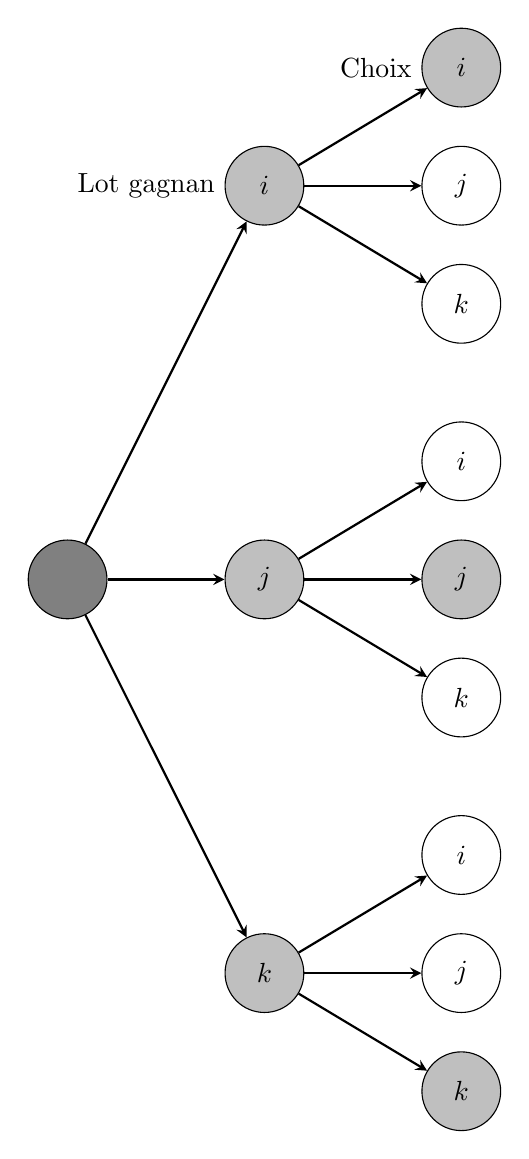
\begin{tikzpicture}
    \tikzstyle{arrow} = [thick,->,>=stealth]
    % Left-most circle
    \node [draw, circle, minimum size=1cm, fill=gray] (Left) at (-5,0) {};

    % One step to the right, top circle
    \node [draw, circle, minimum size=1cm, fill=lightgray, text centered,
           label={-180:Lot gagnan}] (MidTop) at (-2.5,5) {{$\boldsymbol{i}$}};
    \draw [arrow] (Left) -- (MidTop);

      % Two steps to the right, MidTop is parent, top circle
      \node [draw, circle, minimum size=1cm, fill=lightgray, text centered,
             label={-180:Choix}] (MidTopTop) at (0,6.5) {$\boldsymbol{i}$};
      \draw [arrow] (MidTop) -- (MidTopTop);

      % Two steps to the right, MidTop is parent, mid circle
      \node [draw, circle, minimum size=1cm] (MidTopMid) at (0,5) {$j$};
      \draw [arrow] (MidTop) -- (MidTopMid);

      % Two steps to the right, MidTop is parent, bottom circle
      \node [draw, circle, minimum size=1cm] (MidTopBottom) at (0,3.5) {$k$};
      \draw [arrow] (MidTop) -- (MidTopBottom);

    % One step to the right, middle circle
    \node [draw, circle, minimum size=1cm, fill=lightgray] (MidMid) at (-2.5,0) {$\boldsymbol{j}$};
    \draw [arrow] (Left) -- (MidMid);

      % Two steps to the right, MidMid is parent, top circle
      \node [draw, circle, minimum size=1cm] (MidMidTop) at (0,1.5) {$i$};
      \draw [arrow] (MidMid) -- (MidMidTop);

      % Two steps to the right, MidMid is parent, mid circle
      \node [draw, circle, minimum size=1cm, fill=lightgray] (MidMidMid) at (0,0) {$\boldsymbol{j}$};
      \draw [arrow] (MidMid) -- (MidMidMid);

      % Two steps to the right, MidMid is parent, bottom circle
      \node [draw, circle, minimum size=1cm] (MidMidBottom) at (0,-1.5) {$k$};
      \draw [arrow] (MidMid) -- (MidMidBottom);

    % One step to the right, bottom circle
    \node [draw, circle, minimum size=1cm, fill=lightgray] (MidBottom) at (-2.5,-5) {$\boldsymbol{k}$};
    \draw [arrow] (Left) -- (MidBottom);

      % Two steps to the right, MidBottom is parent, top circle
      \node [draw, circle, minimum size=1cm] (MidBottomTop) at (0,-3.5) {$i$};
      \draw [arrow] (MidBottom) -- (MidBottomTop);

      % Two steps to the right, MidBottom is parent, mid circle
      \node [draw, circle, minimum size=1cm] (MidBottomMid) at (0,-5) {$j$};
      \draw [arrow] (MidBottom) -- (MidBottomMid);

      % Two steps to the right, MidBottom is parent, bottom circle
      \node [draw, circle, minimum size=1cm, fill=lightgray] (MidBottomBottom) at (0,-6.5) {$\boldsymbol{k}$};
      \draw [arrow] (MidBottom) -- (MidBottomBottom);
\end{tikzpicture}

